\documentclass{article}

\usepackage[brazil]{babel}  % Define o idioma para português do Brasil

\usepackage{graphicx}       % Pacote para inserção de imagens
\usepackage{hyperref}       % Pacote para links clicáveis
\usepackage{enumitem}       % Pacote para personalização de listas

\usepackage{geometry}       % Pacote para ajustar margens

\geometry{                  % Definindo margens personalizadas (em centímetros)
  left=2.5cm,  % Margem esquerda
  right=2.5cm, % Margem direita
  top=2.5cm,   % Margem superior
  bottom=2.5cm % Margem inferior
}

\usepackage[backend=biber,style=ieee]{biblatex}     % Estilo ieee para bibliografia numerada
\addbibresource{ref.bib}                            % Arquivo .bib


\begin{document}

\begin{titlepage}
    \centering
    % Cabeçalho personalizado
    
\includegraphics[width=0.3\textwidth]{../Topic1/Avaliativo/Imagens/Logo UFLA - Colorida chapada.png}

    \vspace*{2cm} % Espaçamento vertical antes do cabeçalho
    \Large
    Universidade Federal de Lavras\\
    PPGCC\\
    PCC508 – Sistemas Operacionais\\
    
    \vspace{2cm} % Espaço entre o cabeçalho e o título
    \huge % Define o tamanho da fonte do título
    \textbf{Lista Avaliativa 2}
    
    \vfill % Adiciona um espaçamento flexível antes do rodapé (opcional)
    
    % Opcionalmente, você pode incluir seu nome e a data aqui
    \large
    Douglas Aquino T. Mendes\\
    \today % Insere a data atual
\end{titlepage}

\tableofcontents
\newpage

\section{Perguntas}
\subsection{Condições para um processo mudar o estado}
\textbf{Pergunta:} Explique quais são as condições para um processo passar do estado bloqueado para o executando.\newline

\textbf{Resposta:} Para que um processo passe do estado bloqueado para o estado executando, o processo deve estar bloqueado aguardando um evento específico, como a conclusão de uma operação de I/O (entrada/saída) ou a liberação de um recurso. Esse evento deve ocorrer, sinalizando que a condição que causou o bloqueio não está mais presente. Além disso o sistema operacional deve garantir que um processador esteja disponível para agendar o processo. Um processo bloqueado pode não ser selecionado para execução se houver processos com prioridade mais alta que também estejam prontos para serem executados. Após a verificação dessas condições, o sistema operacional realiza a transição do estado do processo de bloqueado para pronto, como é ilustrado na Figura \ref{fig:1}. Se o processo for escolhido pelo escalonador, ele então transita para o estado executando. \cite{borges2024} \cite{tanenbaum2021}

\begin{figure}[h] % 'h' indica que a figura deve ser posicionada aqui, no texto
    \centering % centraliza a imagem
    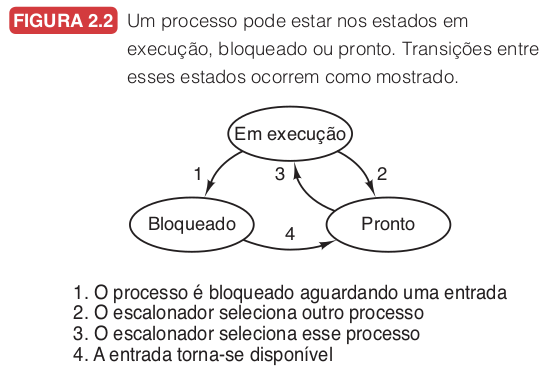
\includegraphics[width=0.5\textwidth]{Images/imageLivroEstadoProcessos.png}
    \caption{Figura 2.2 Reproduzido de Andrew S. Tanenbaum and Herbert Bos (2021) \cite{tanenbaum2021}}
    \label{fig:1} % etiqueta para referência cruzada
\end{figure}

\subsection{Principais informações armazenadas na entrada de um processo}
\textbf{Pergunta:} Explique quais são as principais informações armazenadas na entrada de um processo na tabela de processos. Indique o motivo destas informações.\newline

\textbf{Resposta:} A tabela de processos é uma estrutura de dados mantida pelo sistema operacional que contém informações essenciais sobre cada processo em execução, incluindo o seu contador de programa, ponteiro de pilha, alocação de memória, estado dos arquivos abertos, informação sobre sua contabilidade e escalonamento e tudo o mais que deva ser salvo quando
o processo é trocado do estado em execução para pronto ou bloqueado, de maneira que ele possa ser reiniciado mais tarde como se nunca tivesse sido parado. A Figura \ref{fig:2} \cite{tanenbaum2021} mostra alguns dos campos fundamentais em um sistema típico: os campos na primeira coluna relacionam-se ao gerenciamento de processo. Os outros dois relacionam-se ao gerenciamento de memória e de arquivos, respectivamente. Deve-se observar que precisamente quais campos cada tabela de processo tem é algo altamente dependente do sistema, mas esse número dá uma ideia geral dos tipos de informações necessárias \cite{tanenbaum2021}.

\begin{figure}[h] % 'h' indica que a figura deve ser posicionada aqui, no texto
    \centering % centraliza a imagem
    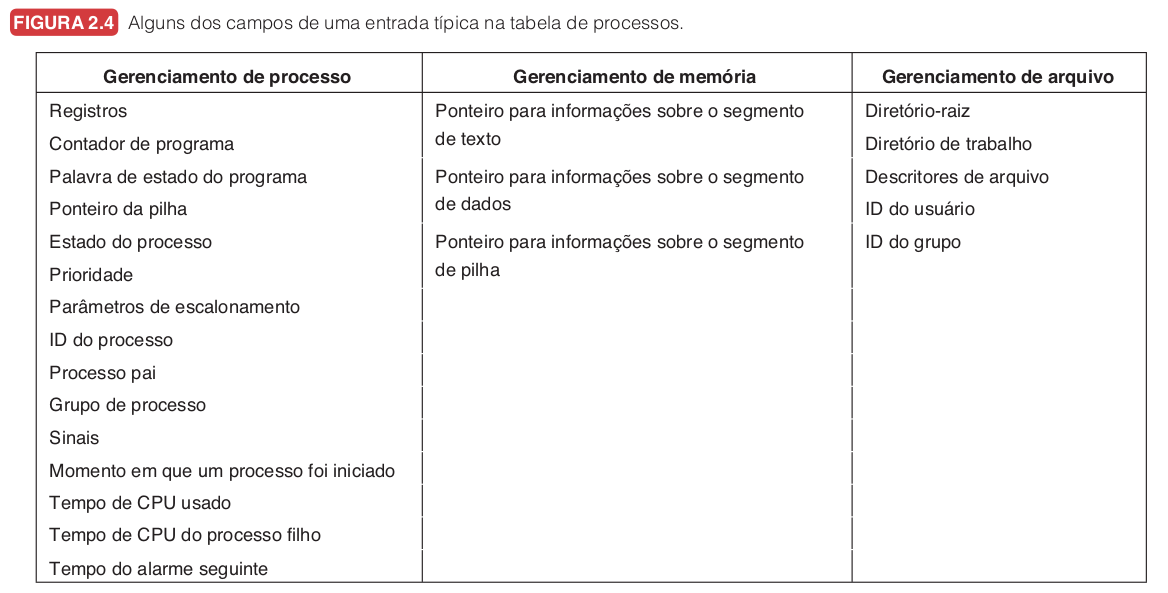
\includegraphics[width=0.9\textwidth]{Images/Captura de tela de 2024-10-18 15-19-09.png}
    \caption{Figura 2.4 Reproduzido de Andrew S. Tanenbaum and Herbert Bos (2021) \cite{tanenbaum2021}}
    \label{fig:2} % etiqueta para referência cruzada
\end{figure}
\newpage

\subsection{Diferença entre processos e threads}
\textbf{Pergunta:} Explique a diferença entre processos e threads, indicando quais itens são únicos por processo e quais por threads.\newline

\textbf{Resposta:} Um processo é uma instância de um programa em execução. Ele é uma unidade de alocação de recursos e possui seu próprio espaço de memória, estado e recursos do sistema. Já uma thread, é a menor unidade de execução dentro de um processo. As threads compartilham o mesmo espaço de memória e recursos do processo ao qual pertencem, permitindo uma comunicação mais eficiente entre elas.

\subsection{Threads implementadas dentro do kernel ou como uma biblioteca}
\textbf{Pergunta:} As threads podem ser implementadas dentro do kernel ou como uma biblioteca no espaço de usuário. Explique a diferença, as vantagens e desvantagens de cada um dos métodos.\newline

\textbf{Resposta:} As threads no Kernel são gerenciadas diretamente pelo sistema operacional, que possui conhecimento sobre a sua existência e estado. O kernel é responsável por realizar todas as operações de gerenciamento de threads, como criação, agendamento e sincronização. Uma das vantagens é que Threads em nível de kernel podem ser agendadas em diferentes processadores em sistemas multiprocessadores, permitindo melhor utilização dos recursos de hardware, já a desvantagem é que o gerenciamento de threads pelo kernel pode introduzir uma sobrecarga maior, já que as operações de criação, destruição e troca de contexto envolvem chamadas de sistema.


As threads no Espaço do Usuário são gerenciadas por uma biblioteca no espaço do usuário, que não envolve o kernel. O sistema operacional não tem conhecimento sobre a existência dessas threads, tratando o processo que contém essas threads como uma única unidade. A vantagem disso é que geralmente é mais leve, pois não requer chamadas de sistema para operações comuns, como criação e destruição de threads. Porém o sistema operacional não tem conhecimento das threads no espaço do usuário, o que limita a capacidade de agendá-las em múltiplos processadores, fazendo com que elas sejam executadas sequencialmente em um único núcleo \cite{geeksforgeeks2024}.


\section{Desenvolver um programa}
\subsection{05) Imprimir na tela os pids recebidos}
\textbf{Enunciado:} Crie um programa que inicialmente cria 4 processos filhos (com fork) formando um conjunto de 5 processos (processo pai e 4 processos filhos). Cada processo filho cria 3 threads. Cada thread dorme um tempo aleatório entre 2 e 10 segundos e termina. O processo filho deve esperar todas as threads terminarem, enviar o seu pid para o processo pai e aí também terminar. O processo pai deve receber o pid dos 3 filhos, esperar todos os processos filhos terminarem e imprimir na tela os pids recebidos e o tempo total transcorrido desde o início. Após isso, deve também terminar. A comunicação dos filhos com o pai será feita utilizando um pipe.\newline

\subsection{06) Lê uma imagem de um arquivo}
\textbf{Enunciado:} O código encontrado no arquivo codigoexercicio.c lê uma imagem de um arquivo, aplica um filtro de convolução em cada canal de cor da imagem e salva novamente a imagem em um outro arquivo. O código utiliza a biblioteca stb e deve ser compilado com: gcc programa.c -lm Modifique o código para que o processamento de cada um dos canais seja processado por uma thread independente. Utilize para isso as threads POSIX. Observação: a biblioteca stb deve estar instalada para que seja possível compilar o código. Consulte o professor para maiores detalhes.\newline

\printbibliography % Imprime a lista de referências

\end{document}